% Cantor's diagonal argument on a list of binary sequences. Generated by a short script.
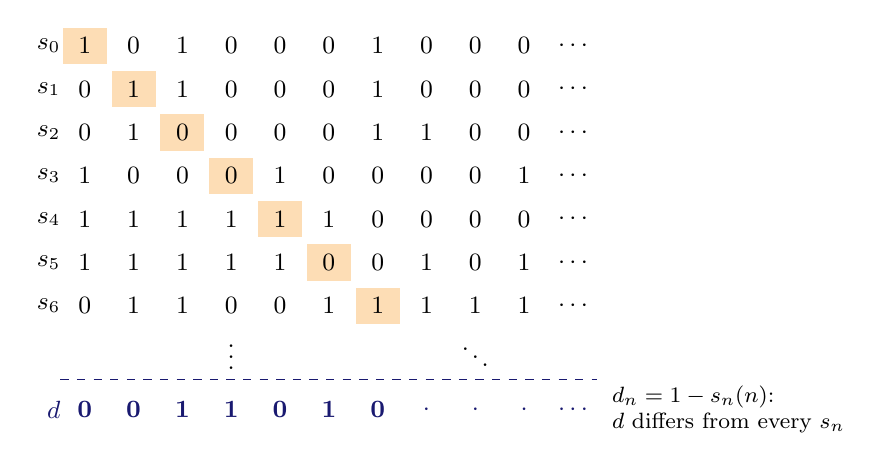
\begin{tikzpicture}[x=0.62cm,y=0.55cm,every node/.style={font=\small}]
\node[left] at (-0.3,0.00) {$s_0$};
\fill[BurntOrange!25] (-0.45,-0.42) rectangle (0.45,0.42);
\node at (0,0) {1};
\node at (1,0) {0};
\node at (2,0) {1};
\node at (3,0) {0};
\node at (4,0) {0};
\node at (5,0) {0};
\node at (6,0) {1};
\node at (7,0) {0};
\node at (8,0) {0};
\node at (9,0) {0};
\node at (10,0) {$\cdots$};
\node[left] at (-0.3,-1.00) {$s_1$};
\node at (0,-1) {0};
\fill[BurntOrange!25] (0.55,-1.42) rectangle (1.45,-0.58);
\node at (1,-1) {1};
\node at (2,-1) {1};
\node at (3,-1) {0};
\node at (4,-1) {0};
\node at (5,-1) {0};
\node at (6,-1) {1};
\node at (7,-1) {0};
\node at (8,-1) {0};
\node at (9,-1) {0};
\node at (10,-1) {$\cdots$};
\node[left] at (-0.3,-2.00) {$s_2$};
\node at (0,-2) {0};
\node at (1,-2) {1};
\fill[BurntOrange!25] (1.55,-2.42) rectangle (2.45,-1.58);
\node at (2,-2) {0};
\node at (3,-2) {0};
\node at (4,-2) {0};
\node at (5,-2) {0};
\node at (6,-2) {1};
\node at (7,-2) {1};
\node at (8,-2) {0};
\node at (9,-2) {0};
\node at (10,-2) {$\cdots$};
\node[left] at (-0.3,-3.00) {$s_3$};
\node at (0,-3) {1};
\node at (1,-3) {0};
\node at (2,-3) {0};
\fill[BurntOrange!25] (2.55,-3.42) rectangle (3.45,-2.58);
\node at (3,-3) {0};
\node at (4,-3) {1};
\node at (5,-3) {0};
\node at (6,-3) {0};
\node at (7,-3) {0};
\node at (8,-3) {0};
\node at (9,-3) {1};
\node at (10,-3) {$\cdots$};
\node[left] at (-0.3,-4.00) {$s_4$};
\node at (0,-4) {1};
\node at (1,-4) {1};
\node at (2,-4) {1};
\node at (3,-4) {1};
\fill[BurntOrange!25] (3.55,-4.42) rectangle (4.45,-3.58);
\node at (4,-4) {1};
\node at (5,-4) {1};
\node at (6,-4) {0};
\node at (7,-4) {0};
\node at (8,-4) {0};
\node at (9,-4) {0};
\node at (10,-4) {$\cdots$};
\node[left] at (-0.3,-5.00) {$s_5$};
\node at (0,-5) {1};
\node at (1,-5) {1};
\node at (2,-5) {1};
\node at (3,-5) {1};
\node at (4,-5) {1};
\fill[BurntOrange!25] (4.55,-5.42) rectangle (5.45,-4.58);
\node at (5,-5) {0};
\node at (6,-5) {0};
\node at (7,-5) {1};
\node at (8,-5) {0};
\node at (9,-5) {1};
\node at (10,-5) {$\cdots$};
\node[left] at (-0.3,-6.00) {$s_6$};
\node at (0,-6) {0};
\node at (1,-6) {1};
\node at (2,-6) {1};
\node at (3,-6) {0};
\node at (4,-6) {0};
\node at (5,-6) {1};
\fill[BurntOrange!25] (5.55,-6.42) rectangle (6.45,-5.58);
\node at (6,-6) {1};
\node at (7,-6) {1};
\node at (8,-6) {1};
\node at (9,-6) {1};
\node at (10,-6) {$\cdots$};
\node at (3,-7) {$\vdots$};
\node at (8,-7) {$\ddots$};
\node[left,MidnightBlue] at (-0.3,-8.40) {$d$};
\node[MidnightBlue,font=\small\bfseries] at (0,-8.40) {0};
\node[MidnightBlue,font=\small\bfseries] at (1,-8.40) {0};
\node[MidnightBlue,font=\small\bfseries] at (2,-8.40) {1};
\node[MidnightBlue,font=\small\bfseries] at (3,-8.40) {1};
\node[MidnightBlue,font=\small\bfseries] at (4,-8.40) {0};
\node[MidnightBlue,font=\small\bfseries] at (5,-8.40) {1};
\node[MidnightBlue,font=\small\bfseries] at (6,-8.40) {0};
\node[MidnightBlue] at (7,-8.40) {$\cdot$};
\node[MidnightBlue] at (8,-8.40) {$\cdot$};
\node[MidnightBlue] at (9,-8.40) {$\cdot$};
\node[MidnightBlue] at (10,-8.40) {$\cdots$};
\draw[MidnightBlue,dashed] (-0.5,-7.70)--(10.50,-7.70);
\node[right,font=\footnotesize,align=left] at (10.60,-8.40) {$d_n=1-s_n(n)$:\\ $d$ differs from every $s_n$};
\end{tikzpicture}
